% Options for packages loaded elsewhere
\PassOptionsToPackage{unicode}{hyperref}
\PassOptionsToPackage{hyphens}{url}
\PassOptionsToPackage{dvipsnames,svgnames,x11names}{xcolor}
%
\documentclass[
  authoryear,
  preprint,
  1p,
  onecolumn]{elsarticle}

\usepackage{amsmath,amssymb}
\usepackage{iftex}
\ifPDFTeX
  \usepackage[T1]{fontenc}
  \usepackage[utf8]{inputenc}
  \usepackage{textcomp} % provide euro and other symbols
\else % if luatex or xetex
  \usepackage{unicode-math}
  \defaultfontfeatures{Scale=MatchLowercase}
  \defaultfontfeatures[\rmfamily]{Ligatures=TeX,Scale=1}
\fi
\usepackage{lmodern}
\ifPDFTeX\else  
    % xetex/luatex font selection
\fi
% Use upquote if available, for straight quotes in verbatim environments
\IfFileExists{upquote.sty}{\usepackage{upquote}}{}
\IfFileExists{microtype.sty}{% use microtype if available
  \usepackage[]{microtype}
  \UseMicrotypeSet[protrusion]{basicmath} % disable protrusion for tt fonts
}{}
\makeatletter
\@ifundefined{KOMAClassName}{% if non-KOMA class
  \IfFileExists{parskip.sty}{%
    \usepackage{parskip}
  }{% else
    \setlength{\parindent}{0pt}
    \setlength{\parskip}{6pt plus 2pt minus 1pt}}
}{% if KOMA class
  \KOMAoptions{parskip=half}}
\makeatother
\usepackage{xcolor}
\setlength{\emergencystretch}{3em} % prevent overfull lines
\setcounter{secnumdepth}{5}
% Make \paragraph and \subparagraph free-standing
\makeatletter
\ifx\paragraph\undefined\else
  \let\oldparagraph\paragraph
  \renewcommand{\paragraph}{
    \@ifstar
      \xxxParagraphStar
      \xxxParagraphNoStar
  }
  \newcommand{\xxxParagraphStar}[1]{\oldparagraph*{#1}\mbox{}}
  \newcommand{\xxxParagraphNoStar}[1]{\oldparagraph{#1}\mbox{}}
\fi
\ifx\subparagraph\undefined\else
  \let\oldsubparagraph\subparagraph
  \renewcommand{\subparagraph}{
    \@ifstar
      \xxxSubParagraphStar
      \xxxSubParagraphNoStar
  }
  \newcommand{\xxxSubParagraphStar}[1]{\oldsubparagraph*{#1}\mbox{}}
  \newcommand{\xxxSubParagraphNoStar}[1]{\oldsubparagraph{#1}\mbox{}}
\fi
\makeatother


\providecommand{\tightlist}{%
  \setlength{\itemsep}{0pt}\setlength{\parskip}{0pt}}\usepackage{longtable,booktabs,array}
\usepackage{calc} % for calculating minipage widths
% Correct order of tables after \paragraph or \subparagraph
\usepackage{etoolbox}
\makeatletter
\patchcmd\longtable{\par}{\if@noskipsec\mbox{}\fi\par}{}{}
\makeatother
% Allow footnotes in longtable head/foot
\IfFileExists{footnotehyper.sty}{\usepackage{footnotehyper}}{\usepackage{footnote}}
\makesavenoteenv{longtable}
\usepackage{graphicx}
\makeatletter
\def\maxwidth{\ifdim\Gin@nat@width>\linewidth\linewidth\else\Gin@nat@width\fi}
\def\maxheight{\ifdim\Gin@nat@height>\textheight\textheight\else\Gin@nat@height\fi}
\makeatother
% Scale images if necessary, so that they will not overflow the page
% margins by default, and it is still possible to overwrite the defaults
% using explicit options in \includegraphics[width, height, ...]{}
\setkeys{Gin}{width=\maxwidth,height=\maxheight,keepaspectratio}
% Set default figure placement to htbp
\makeatletter
\def\fps@figure{htbp}
\makeatother

\makeatletter
\@ifpackageloaded{float}{}{\usepackage{float}}
\floatstyle{plain}
\@ifundefined{c@chapter}{\newfloat{suppfig}{h}{losuppfig}}{\newfloat{suppfig}{h}{losuppfig}[chapter]}
\floatname{suppfig}{Figure S}
\newcommand*\quartosuppfigref[1]{Figure \hyperref[#1]{S\ref{#1}}}
\@ifpackageloaded{caption}{}{\usepackage{caption}}
\DeclareCaptionLabelFormat{quartosuppfigreflabelformat}{#1#2}
\captionsetup[suppfig]{labelformat=quartosuppfigreflabelformat}
\newcommand*\listofsuppfigs{\listof{suppfig}{List of Supplementary Figures}}
\makeatother
\makeatletter
\@ifpackageloaded{caption}{}{\usepackage{caption}}
\AtBeginDocument{%
\ifdefined\contentsname
  \renewcommand*\contentsname{Table of contents}
\else
  \newcommand\contentsname{Table of contents}
\fi
\ifdefined\listfigurename
  \renewcommand*\listfigurename{List of Figures}
\else
  \newcommand\listfigurename{List of Figures}
\fi
\ifdefined\listtablename
  \renewcommand*\listtablename{List of Tables}
\else
  \newcommand\listtablename{List of Tables}
\fi
\ifdefined\figurename
  \renewcommand*\figurename{Figure}
\else
  \newcommand\figurename{Figure}
\fi
\ifdefined\tablename
  \renewcommand*\tablename{Table}
\else
  \newcommand\tablename{Table}
\fi
}
\@ifpackageloaded{float}{}{\usepackage{float}}
\floatstyle{ruled}
\@ifundefined{c@chapter}{\newfloat{codelisting}{h}{lop}}{\newfloat{codelisting}{h}{lop}[chapter]}
\floatname{codelisting}{Listing}
\newcommand*\listoflistings{\listof{codelisting}{List of Listings}}
\makeatother
\makeatletter
\makeatother
\makeatletter
\@ifpackageloaded{caption}{}{\usepackage{caption}}
\@ifpackageloaded{subcaption}{}{\usepackage{subcaption}}
\makeatother
\journal{Journal of Hydrology}

\ifLuaTeX
  \usepackage{selnolig}  % disable illegal ligatures
\fi
\usepackage[]{natbib}
\bibliographystyle{elsarticle-harv}
\usepackage{bookmark}

\IfFileExists{xurl.sty}{\usepackage{xurl}}{} % add URL line breaks if available
\urlstyle{same} % disable monospaced font for URLs
\hypersetup{
  pdftitle={Regional Base-Flow Index in Arid Landscapes Using Machine Learning and Instrumented Records},
  pdfauthor={Caelum Mroczek; Abraham E Springer; Neha Gupta; Temuulen Sankey; Benjamin Lucas},
  colorlinks=true,
  linkcolor={blue},
  filecolor={Maroon},
  citecolor={Blue},
  urlcolor={Blue},
  pdfcreator={LaTeX via pandoc}}


\setlength{\parindent}{6pt}
\begin{document}

\begin{frontmatter}
\title{Regional Base-Flow Index in Arid Landscapes Using Machine
Learning and Instrumented Records}
\author[1]{Caelum Mroczek%
\corref{cor1}%
}
 \ead{csm428@nau.edu} 
\author[1]{Abraham E Springer%
%
}

\author[2]{Neha Gupta%
%
}

\author[3]{Temuulen Sankey%
%
}

\author[4]{Benjamin Lucas%
%
}


\affiliation[1]{organization={School of Earth and Sustainability,
Northern Arizona University, Flagstaff, AZ, USA},,postcodesep={}}
\affiliation[2]{organization={Department of Hydrology and Atmospheric
Sciences, University of Arizona, Tucson, AZ, USA},,postcodesep={}}
\affiliation[3]{organization={School of Informatics, Computing, and
Cyber Systems, Northern Arizona University, Flagstaff, AZ,
USA},,postcodesep={}}
\affiliation[4]{organization={Department of Mathematics and Statistics,
Northern Arizona University, Flagstaff, AZ, USA},,postcodesep={}}

\cortext[cor1]{Corresponding author}





        
\begin{abstract}
Base flow, sustained by groundwater discharge, is a vital component of
river ecosystems, particularly in drylands, where water resources are
limited. This novel study analyzes the instrumented streamflow record in
Arizona to assess long-term base-flow index (BFI) trends across gauged
catchments. Results indicate that approximately 32\% of Arizona's
streamflow originates from groundwater discharge, with significant
spatial variability driven by landscape and climatic factors. Base-flow
relationships are analyzed with coincident trends in climate variables
such as precipitation, evapotranspiration, and temperature. Spatial and
climatic trends reveal variability in base-flow contributions, providing
insight into groundwater-surface water interactions in arid and
semi-arid landscapes. Building on this analysis, we applied machine
learning methods to predict BFI in ungauged basins, addressing the
challenges of Arizona's sparse streamgage network. Using the eXtreme
Gradient Boosting (XGBoost) algorithm trained on hydroclimate and
physiographic predictors, we estimated long-term BFI from 1991 to 2020.
This combined approach integrates observational data with predictive
modeling to enhance our understanding of base-flow processes and provide
a framework for water resource management in data-limited regions.
\end{abstract}





\end{frontmatter}
    

\subsection{Key Points}\label{key-points}

\begin{itemize}
\tightlist
\item
  Approximately 32\% of Arizona's streamflow originates from groundwater
  discharge.
\item
  XGBoost predicted long-term BFI in ungauged basins, filling dryland
  data gaps.
\item
  Baseflow trends track precipitation, emphasizing climate's role in
  dryland hydrology.
\end{itemize}

\section{Introduction}\label{sec-intro}

Dryland regions, encompassing arid, semi-arid, hyper-arid, and dry
sub-humid systems, cover 40\% of the Earth's land surface. These regions
are home to approximately 2 billion people globally and constitute the
largest terrestrial biome \citep{iucn-drylands-2019}. Despite supporting
diverse ecosystems and human populations, dryland regions face mounting
hydrologic challenges exacerbated by increasing urbanization, expanding
agricultural activities, and climate-induced amplification of
precipitation patterns \citep{taylor2013}. This water scarcity is
intensifying due to the compounding effects of climate variability and
increased groundwater extraction \citep{taylor2013}. Groundwater serves
as a vital resource in drylands for sustaining ecological functions and
supporting human livelihoods \citep{scanlon2006, yao2018}.

Base flow is the sustained portion of streamflow in the absence of
runoff that is derived from groundwater discharge
\citep{usgs-glossary-2018}. Base flow is critical to maintaining
seasonal low-flow regimes, supporting aquatic ecosystems, and
facilitating the transport of nutrients and chemicals. Base-flow
contribution to streamflow can be highly variable spatially
\citep{singh2018, bosch2017, beck2013}, and temporally
\citep{ficklin2016, tan2020}. Increasing groundwater extraction, changes
in land cover/land use, and changes in precipitation patterns due to
climate change affect the timing and volumes of base flow
\citep{tan2020, taylor2013}. Effective management of water quantity and
quality depends on understanding seasonal and interannual base-flow
patterns and long-term changes in base-flow behavior.

The Base-Flow Index (BFI) is the ratio of the long-term mean base-flow
volume to the long-term total streamflow volume expressed as a
percentage. BFI serves as a normalized measure of groundwater
contribution interannually or between basins. BFI is determined by
hydrograph separation and is influenced by the climate and physiographic
characteristics of a catchment \citep{neff2005, beck2013, singh2018}.
Between catchments, base flow fluctuates according to changes in the
moisture content of the vadose zone, influenced by varying levels of
evapotranspiration and aquifer storage dynamics \citep{bosch2017}. Since
BFI calculations rely on instrumented stream records, it remains unknown
for ungauged catchments, which encompass most of the earth's land
surface \citep{fekete2007}. Addressing this information gap is integral
to approaching a comprehensive understanding of groundwater dynamics
globally. This study addresses this gap by analyzing long-term BFI
patterns across Arizona using instrumented streamflow records and
applying a machine learning model to predict BFI in ungauged catchments.

Advancements in machine learning provide tools to predict hydrologic
indices in ungauged basins, addressing the limitations of sparse
streamgage networks. To tackle the challenge of quantifying base-flow
indices in ungauged catchments, numerous studies have applied both
regression and machine learning methods. \citet{ahiablame2013} found
that using a regression model to estimate annual base flow of ungauged
catchments was reasonably easy and accurate. \citet{beck2013} overcame
the nonlinearity of basin characteristics and improved results of
multivariate analyses by using artificial neural networks (ANN) to
estimate BFI globally. \citet{singh2018} implemented a random forest
algorithm to predict long-term BFI for ungauged catchments across New
Zealand. These applications demonstrate the versatility and
effectiveness of machine learning in capturing complex ecohydrologic
dynamics and improving our understanding of groundwater contributions to
streamflow.

Previous studies have examined base-flow regionalization and synthesis
across various spatial scales, from global to continental
\citep{beck2013, santhi2008, ayers2022, singh2018}. Such large-scale
analyses often utilize generalized datasets and methodologies, resulting
in limited applicability to regions with unique hydrogeologic and
climatic conditions. Additionally, global and continental-scale studies
tend to rely on streamgage networks that disproportionately represent
large perennial rivers and regulated watersheds with dense human
populations, while underrepresenting arid and semi-arid regions
characterized by non-perennial flow regimes and smaller streams
\citep{krabbenhoft-2022}. Thus, their effectiveness in accurately
capturing groundwater-surface water interactions, particularly in
critically water-stressed dryland regions, remains constrained.

Despite advancements, existing large-scale studies have limited
applicability to the unique hydrogeologic conditions in arid and
semi-arid regions like Arizona, leaving uncertainty regarding
groundwater-surface water interactions in these critically
water-stressed areas. This study addresses this crucial gap by
developing a regionally tailored machine learning model specifically
designed to estimate BFI for Arizona's ungauged basins. Utilizing
hydrogeologic characteristics and hydroclimatic data, we estimate
long-term mean BFI (1991--2020) in ungauged catchments, filling spatial
gaps in the sparse streamgage network. Furthermore, regional trends in
base flow and BFI at instrumented sites are analyzed alongside
coincident climate trends in precipitation, reference evapotranspiration
(ETO), and temperature. The outcomes offer novel insights into
groundwater contributions to streamflow, supporting water resource
management in an area increasingly vulnerable to drought and climate
change impacts, and contributing broadly to the understanding of
hydrologic processes in dryland environments. The objectives of this
study are to (1) quantify long-term spatial and temporal trends in BFI
across Arizona, and (2) develop a predictive model using eXtreme
Gradient Boosting (XGBoost) to estimate BFI in ungauged basins based on
hydroclimatic and geospatial variables.

\section{Methods}\label{sec-methods}

\subsection{Study Area}\label{sec-study-area}

Arizona, located in the southwestern United States, spans approximately
295,253 km² and encompasses a diverse range of landscapes, elevations,
and climate regimes. The state includes portions of two major
physiographic regions: the Colorado Plateau in the northeast, the Basin
and Range province in the south and west, and a transitional zone, the
Central Highlands, between them. This heterogeneity results in
substantial variation in environmental conditions across the state. The
Colorado Plateau is characterized by high-elevation desert and mountain
woodlands, averaging 1,936 masl (6,352 ft), with mean temperatures
ranging from -6°C (20°F) to 26°C (80°F) and annual precipitation of
about 580 mm (23 in). In contrast, the Basin and Range region is lower
in elevation, averaging 490 masl (1,600 ft), and features a semi-arid to
arid climate, with temperatures ranging from 15°C (60°F) to 43°C (110°F)
and an average annual precipitation of 200 mm (8 in)
\citep{az_climate2024}. The Central Highlands feature a mix of
mountainous terrain and interspersed basins, adding to the state's
topographic and hydroclimatic complexity.

\begin{figure}

\centering{

\includegraphics{images/updated/StudyArea_20250404.png}

}

\caption{\label{fig-study-area}Map of Arizona and US Geological Survey
(USGS) streamgages used in this study. 8-digit HUC subbasin boundaries
and physiographic regions shown.}

\end{figure}%

Arizona's hydrology varies seasonally and spatially between its
physiographic regions. In summer, localized and intense convective
storms stem from the North American Monsoon; in winter, orographic
precipitation is delivered by Pacific frontal systems
\citep{eastoe2019mtnblock}. While monsoonal precipitation can account
for up to 50\% of annual precipitation, evaporation and dry preceding
soil properties leads to most precipitation becoming runoff
\citep{sheppard2002}. As such, 94\% of streams in Arizona are ephemeral
or intermittent \citep{epa_AZephemeral}. Much of the hydrology of
Arizona is snow-melt derived, driven by spring melt from the
high-elevation Colorado Plateau winter snowpack. Though winter
precipitation accounts for only 30\% of annual precipitation totals, it
provides the majority of water for natural reservoirs
\citep{sheppard2002}.

\subsection{Data}\label{sec-data}

Daily observed streamflow data obtained from the United States
Geological Survey (USGS) National Water Information System (NWIS) were
used in this study. Streamgages were selected depending on criteria to
ensure the applicability of each site. Following the findings of
\citet{odonnell2016}, which determined that 8--10 years of calibration
data are necessary to account for climate variability in paired
watershed studies in the region, a minimum record length of 10 years was
required. Additionally, years with more than 30 missing days of
streamflow data were excluded from the analysis. Streamgages directly
downstream of major regulation (e.g., reservoirs, lakes, diversions)
were excluded, based on USGS annual water data reports and site metadata
\citep{usgs2010}. While some flow alteration is widespread, the focus
was on removing gauges with clear, immediate regulatory impacts. As
such, streamgages along the Colorado River were omitted because they
represent managed flows governed by the Colorado River Compact. After
applying these selection criteria, 205 USGS streamgages with acceptable
periods of record were included in the study
(Figure~\ref{fig-study-area}). Periods of record ranged from 10 to 112
years, with a median of 28 years.

Our data selection criteria ensure a robust analysis but also highlight
notable spatial gaps that our machine learning model can address.
Arizona has 184 active USGS streamflow stations (as of 2024) covering an
area of 295,253 km². For comparison, Indiana (a humid state in the U.S.)
maintains 189 active stations within a significantly smaller area of
94,326 km². This results in a streamgage density of approximately 2.004
gauges per 1,000 km² in Indiana, more than three times greater than
Arizona's density of 0.623 gauges per 1,000 km². Such disparities in
gauge coverage are typical for dryland regions globally
\citep{krabbenhoft-2022}, underscoring the necessity and relevance of
this type of modeling approach in arid and semi-arid environments.

Watersheds across the United States are delineated by the USGS using a
hydrologically-defined network. This system delineates the country using
hierarchical hydrologic unit codes (HUCs), where each subsequent basin
includes the digits of the enclosing basin. Here, 8-digit HUCs (HUC 8s)
are used to divide Arizona into 84 sub-basins that are fully or
partially in the state (Figure~\ref{fig-study-area}). These HUC 8
sub-basins are analogous to medium-sized river basins and are defined by
surface water characteristics.

Annual precipitation and temperature data came from the PRISM climate
group at Oregon State University at a resolution of 4 km
(\url{https://prism.oregonstate.edu;} \citep{daly2008}). The PRISM
dataset provides valuable insights into regional climate in ungauged
regions and has been shown to perform well across the southwestern US
\citep{buban_PRISM}. Instead of the water year, PRISM data uses a
calendar-year format, which was adopted for consistency in the water
balance. Although this may introduce challenges in the annual estimates
due to inter-annual snow storage, the use of long-term annual averages
reduces potential errors \citep{reitz2017}.

Annual reference evapotranspiration (ET\textsubscript{O}) data came from
TerraClimate, a 4-km grid climatological data set
\citep{abatzoglou2018}. TerraClimate uses a Penman-Monteith approach to
generate a reference evapotranspiration. The ET\textsubscript{O} values
were calculated assuming a reference grass surface across the landscape
with unlimited water. In the drylands of the southwestern US,
ET\textsubscript{O} typically exceeds precipitation annually
\citep{zomer2022}.

Basin elevation was derived from a 30-meter resolution Digital Elevation
Model (DEM) from the USGS National Elevation Dataset. The DEM of Arizona
was used to derive key basin characteristics: basin area, average slope,
and the proportion of each basin oriented toward north or south aspects.
Various geospatial variables, such as aspect, were disaggregated then
averaged to assess the areal percentage of each sub-variable within
individual HUC 8 basins. By calculating these percentages, we derived a
more comprehensive understanding of landscape composition across space.
Land cover was acquired from USGS-NLCD (National Land Cover Database),
hydrologic soil group from SSURGO (Soil Survey Geographic Database), and
underlying geology and karst from USGS were all similarly averaged
across the basins. Aggregating variables to align with the HUC 8
boundaries allowed for more precise predictions of BFI by integrating
spatial variations within each basin.

\subsection{Base-flow separation}\label{sec-bf_sep}

Directly measuring base flow and base-flow index (BFI) presents unique
challenges \citep{eckhardt2008}. Base flow is a physical hydrologic
process representing groundwater contributions to streamflow, while BFI
is a dimensionless, statistical metric that estimates the proportion of
streamflow derived from base flow. Because BFI must be derived using a
base-flow separation technique, its value is inherently method-dependent
and sensitive to the separation approach used \citep{beck2013}. A
variety of techniques have been developed to estimate base flow,
including tracer studies \citep{gonzales2009}, graphical interpolation
methods \citep{instituteofhydrology1980, sloto1996}, and digital filters
\citep{arnold1995, eckhardt2005, lyne1979, nathan1990}. Each of these
methods varies in its applicability depending on spatial scale, record
length, and study objectives. Although the choice of separation method
and parameterization introduces some subjectivity, these filters have
been shown to yield reliable estimates when applied consistently within
a study domain
\citep{chapman_1999, eckhardt2005, instituteofhydrology1980, ayers2022}.
Numerous studies have compared these separation techniques
\citep[e.g.,][]{eckhardt2005, eckhardt2008, nathan1990}; however, this
study does not evaluate the relative performance of different methods.

Base flow was calculated using a single-parameter, recursive digital
filter technique from \citet{nathan1990}. This base-flow separation
technique is based on a recursive digital filter used in signal analysis
that separates high-frequency signals (quickflow) from low-frequency
signals (base flow) \citep{lyne1979}. \citet{eckhardt2023} noted that
recursive digital filters lack a physical basis, but as the method is
easy to automate, objective, and repeatable, it is appropriate for a
regional-scale study. The Lyne-Hollick filter has been used in multiple
studies \citep{ARNOLD200021, santhi2008, bloomfield2009, singh2018}, and
it takes the form of

\begin{equation}\phantomsection\label{eq-bf-separate}{
b = \alpha b_{k-1} + \frac{1-\alpha}{2}(Q_k + Q_{k-1})
}\end{equation}

where \(b\) is base flow, \(\alpha\) is the filter parameter, \(Q\) is
the total streamflow, and \(k\) is the time step. A filter parameter
\(\alpha\) of 0.925 was used as in \citet{nathan1990} and
\citet{fuka2014ecohydrology}. The filter was run three times (forward,
backward, forward) to attenuate the base-flow signal.

Two BFI metrics were used in this study: (1) annual BFI, calculated for
each calendar year using daily streamflow records, and (2) long-term
BFI, defined as the average of annual BFI values over the period of
record at each site. Annual BFI reflects interannual variability in
base-flow contributions, while long-term BFI represents a time-averaged
metric of groundwater influence. The machine learning model was trained
to predict annual BFI values, which were then aggregated to produce
long-term BFI estimates.

\subsection{Machine Learning}\label{machine-learning}

The implementation of machine learning models to predict hydrologic
indices has been successful in past studies
\citep{singh2018, schmidt_ML_2020, Rozos2021Machine}. In this work, we
used the eXtreme Gradient Boosting (XGBoost) algorithm
\citep{chen2016xgboost} to predict BFI at ungauged locations using
catchment characteristics as predictors Table~\ref{tbl-predictors}. The
XGBoost algorithm is a decision tree-based ensemble algorithm, which can
be adapted for either regression or classification problems. This
algorithm iteratively builds an ensemble of decision trees, where each
tree corrects errors from previous trees to improve predictions
\citep{chen2016xgboost}. Its efficiency, scalability, and robustness
have made it increasingly popular in recent years, with successful
applications in environmental modeling tasks such as streamflow
forecasting \citep{szczepanek2022daily, ni2020streamflow} and land
use/land cover classification \citep{Georganos2018Very}.

XGBoost operates by leveraging gradient boosting on decision tree
algorithms, combining multiple low-variance models to produce a robust
overall prediction. Gradient boosting works iteratively: the initial
tree is trained on the target values, while subsequent trees are trained
on the residual errors of the preceding tree. Each tree is assigned a
weight based on its contribution to reducing error, and these weights
are used to determine the influence of each tree in the final model. The
ultimate prediction is made by aggregating the outputs of all \(n\)
weighted trees in the ensemble. In this study, the trained XGBoost model
is used to predict BFI in ungauged catchments based on geospatial and
hydroclimate predictor variables (Table~\ref{tbl-predictors}). Certain
features were further subdivided according to their areal coverage
within each basin (e.g.~land cover was divided into 16 subdivisions).
This approach allowed the model to capture finer-scale spatial
variability and improve predictive accuracy.

\begin{longtable}[]{@{}llll@{}}
\caption{Basin-characteristic variables used as initial features in
XGBoost model. Starred features are maintained in the final,
dimensionality-reduced model.}\label{tbl-predictors}\tabularnewline
\toprule\noalign{}
& Variable & Source & Geoprocessing \\
\midrule\noalign{}
\endfirsthead
\toprule\noalign{}
& Variable & Source & Geoprocessing \\
\midrule\noalign{}
\endhead
\bottomrule\noalign{}
\endlastfoot
Hydroclimate & Precipitation* & PRISM & Basin average \\
& Mean Temperature* & PRISM & Basin average \\
& Reference Evapotranspiration* & TerraClimate & Basin average \\
Geospatial & Elevation* & DEM & Basin average \\
& Area & DEM & Basin average \\
& Slope & DEM & Basin average \\
& Aspect & DEM & Percent areal coverage \\
& Land Cover* & NLCD & Percent areal coverage \\
& Hydrologic Soil Group* & SSURGO & Percent areal coverage \\
& Geology & USGS & Percent areal coverage \\
& Karst & USGS & Percent areal coverage \\
\end{longtable}

Our training dataset consisted of 7,724 site-year observations of annual
BFI, where each observation represents a single water year at a given
streamgage. These observations were paired with 45 predictor variables
derived from basin characteristics and climate data. To optimize the
model's performance, we first conducted an exhaustive grid search
combined with 5-fold cross-validation to identify the optimal
hyperparameter values. The hyperparameters evaluated included the
learning rate (\(\eta\)), minimum split loss (\(\gamma\)), maximum tree
depth, minimum child weight, and the number of trees. While not an
exhaustive list of all possible XGBoost hyperparameters, this range of
values provided sufficient variation to ensure the selection of a
high-performing model. The optimal hyperparameters were determined to
be: 700 trees, a learning rate (\(\eta\)) of 0.05, a minimum split loss
(\(\gamma\)) of 0.075, a maximum tree depth of 7, and a minimum child
weight of 5. Using these values, the XGBoost model was trained on the
dataset with 10-fold cross-validation.

\(K\)-fold cross-validation provides an unbiased estimate of a model's
accuracy on unseen data, while also insuring against overfitting or
underfitting. In this approach, the data are randomly divided into \(k\)
folds of equal size. The model is trained on \(k-1\) folds and tested on
the remaining fold, referred to as the validation set. This process is
repeated \(k\) times, with each fold serving as the validation set
exactly once. Each iteration trains an independent model with the same
hyperparameters but using a different subset of training data. By
averaging the model performance across all \(k\) folds, we achieve a
robust and reliable estimate of predictive accuracy. Root mean squared
error (RMSE) was used as the performance metric for both model
optimization and evaluation. RMSE provided a consistent and
interpretable measure of the model's accuracy throughout the training
and validation process.

\begin{figure}

\centering{

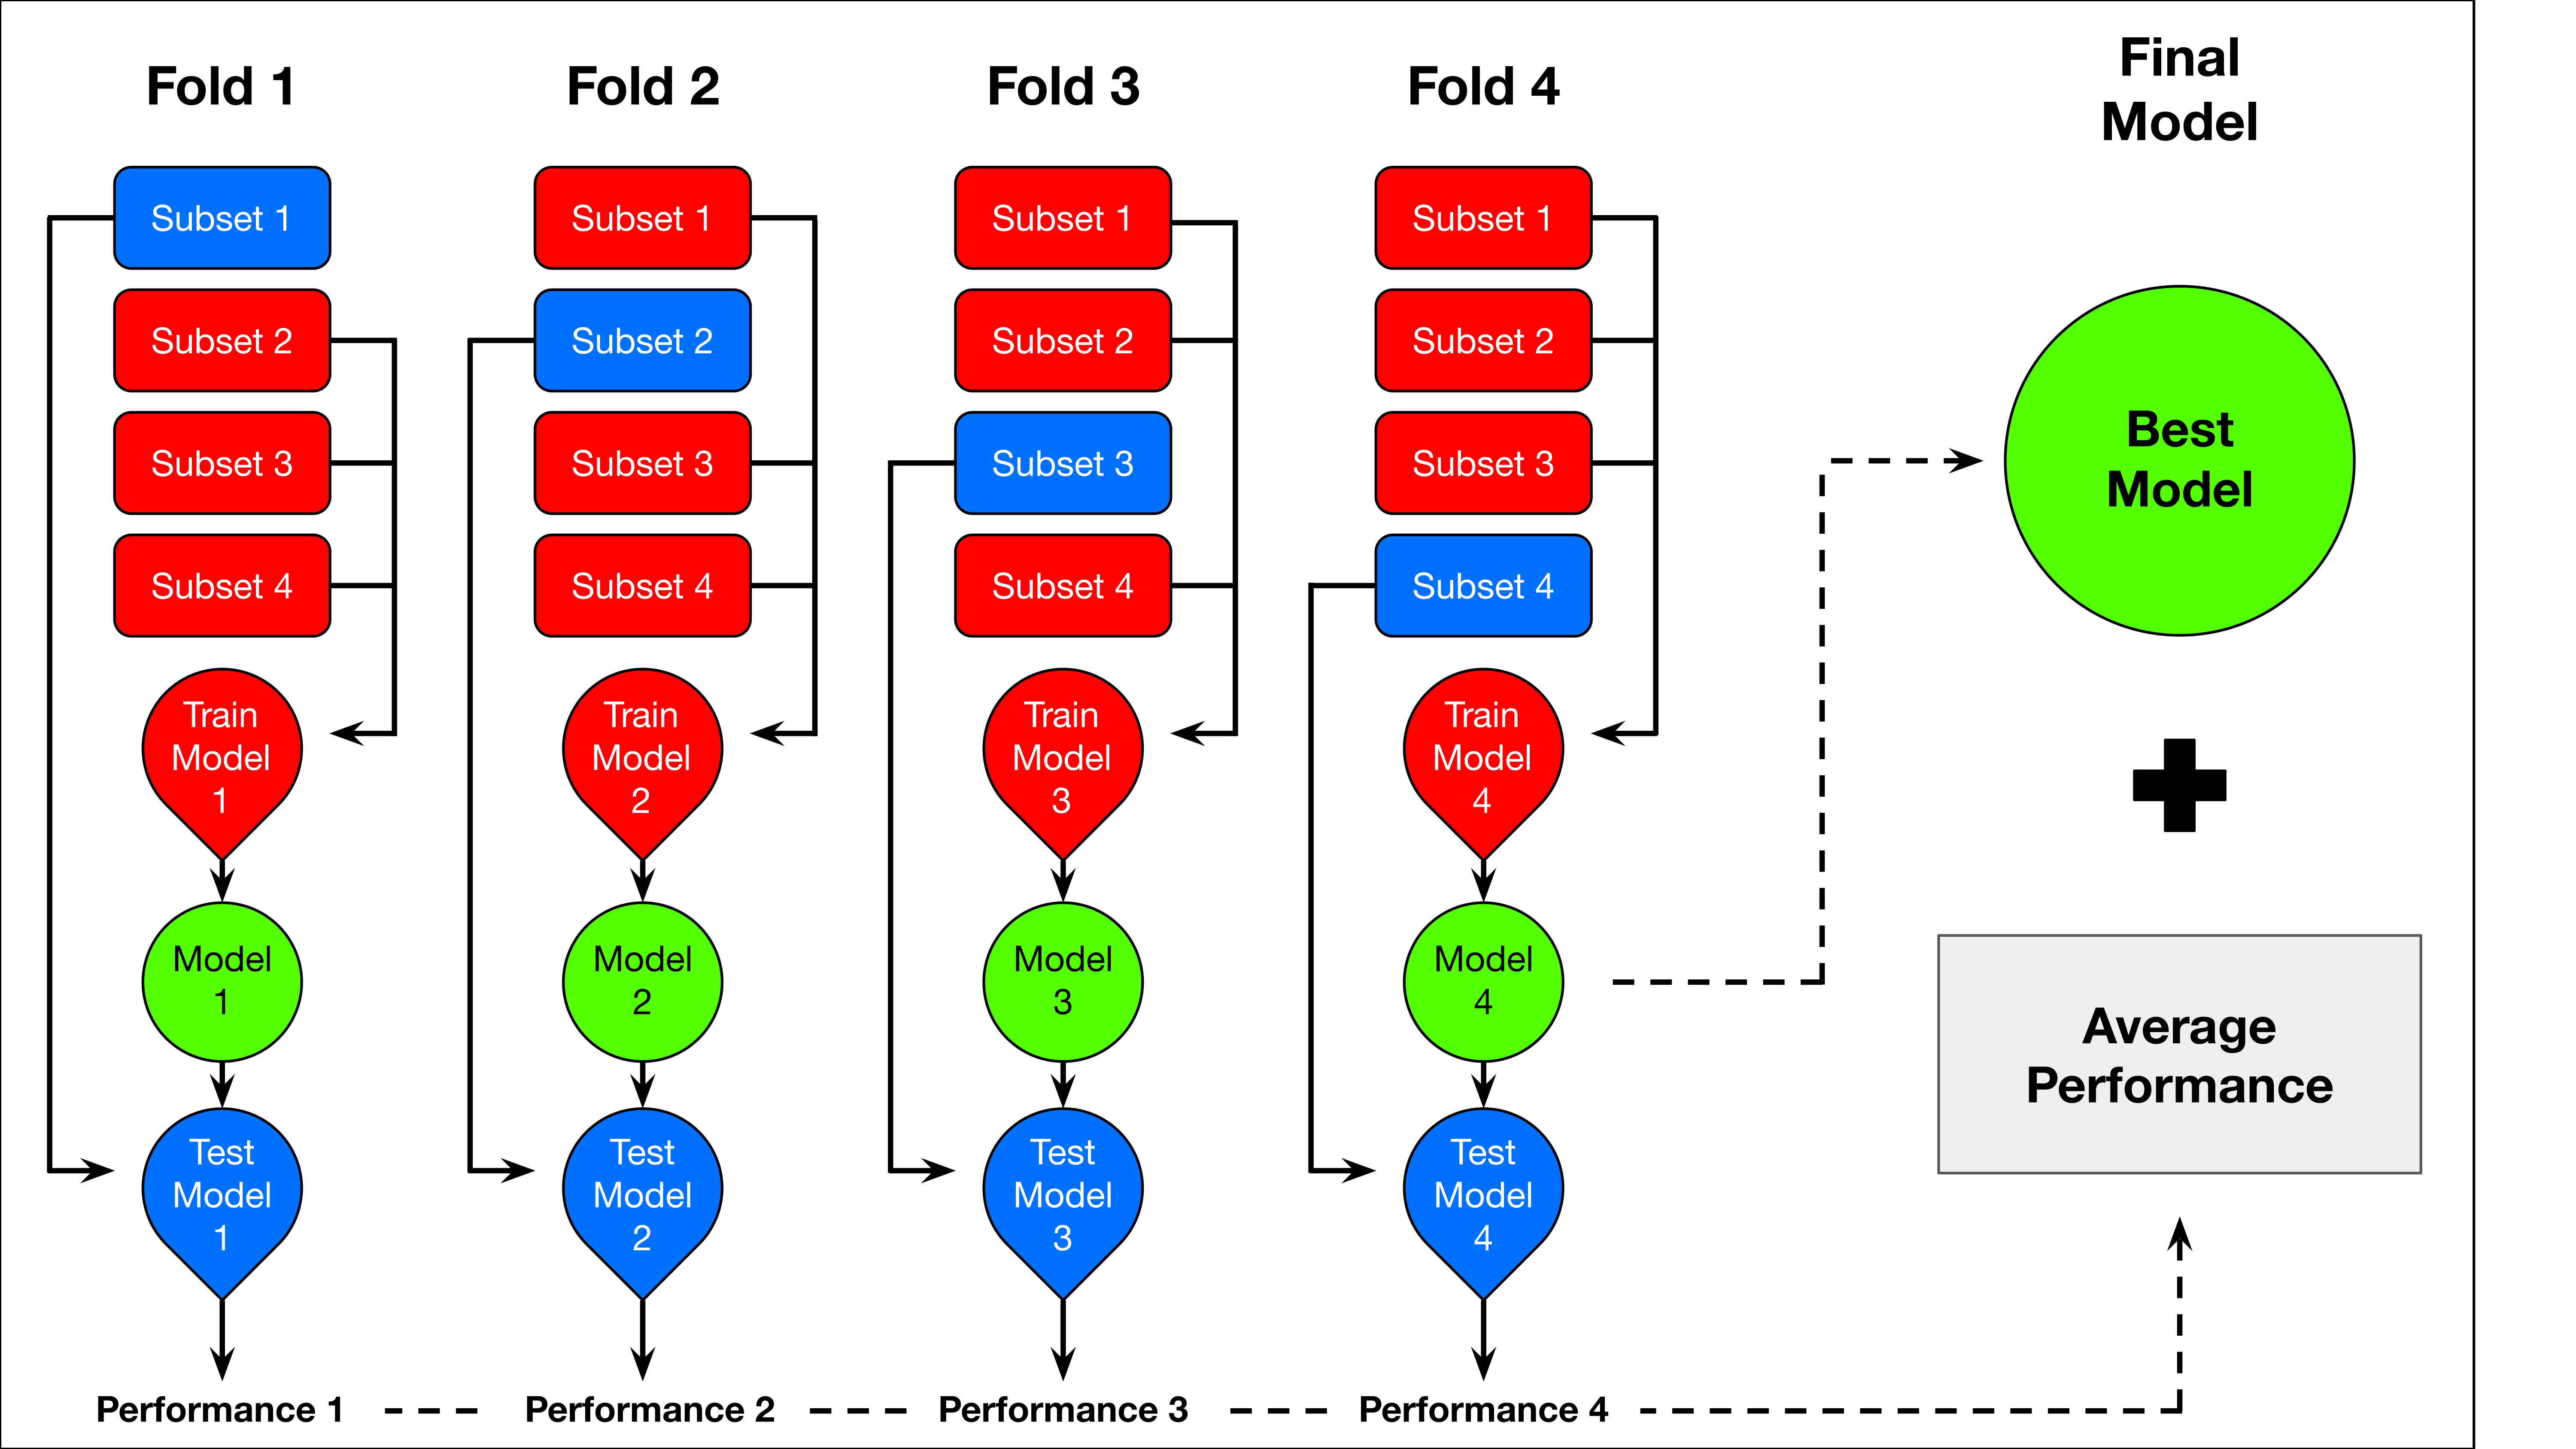
\includegraphics[width=1\textwidth,height=\textheight]{images/k-fold_fig.png}

}

\caption{\label{fig-k-fold}Schematic of \(k\)-fold cross validation. The
dataset is randomly divided into \(k\) stratified folds. Each fold
serves as the validation set once, while the remaining folds are
combined to create a training set for model development. Performance
metrics for the test set are calculated and recorded, and this process
is repeated for all \(k\) folds.}

\end{figure}%

\subsubsection{Feature Selection}\label{sec-feat-selection}

Machine learning models are prone to overfitting, especially when
provided with a large set of predictive features \citep{Ying_2019}.
Overfitting can degrade model performance on unseen data and increase
the demand for computational resources and memory storage
\citep{feat_selec2017}. Dimensionality reduction offers a robust
solution to these challenges and generally falls into two broad
categories: feature extraction and feature selection.

Feature extraction involves transforming the original dataset into a
lower-dimensional feature space. However, this process generates new
features that often lack the physical interpretability of the original
variables. In contrast, feature selection identifies a subset of the
original features, preserving their physical meaning while improving
model readability and interpretability \citep{feat_selec2017}. In this
study, supervised feature selection was employed to reduce the number of
predictors, which enhanced learning performance, reduced computational
costs, and mitigated overfitting.

To begin, an initial model was trained using the full feature set of 45
predictors (Table~\ref{tbl-predictors}). A feature selection method
based on feature importance was then applied to identify and remove less
relevant and noisy features. Feature importance scores quantify the
contribution of individual features---either positively or
negatively---to the model's predictions \citep{ML_interpretability2019}.
In this analysis, SHAP (SHapley Additive exPlanations) values were used
to compute feature importance scores \citep{SHAP_values}.

SHAP values is a method to explain the prediction of an individual
instance by calculating the contribution of each feature to that
prediction. The method is based on coalition game theory and is
discussed further in \citet{SHAP_values}. Here, SHAP values are used for
global interpretation of feature importance and feature effects on the
model. Global feature importance is produced by the absolute Shapley
values of each feature across the dataset, providing a list of features
in order of most to least important. Feature effects provide an
indication of the relationship between the value of a predicting feature
and its impact on the prediction.

\begin{figure}

\centering{

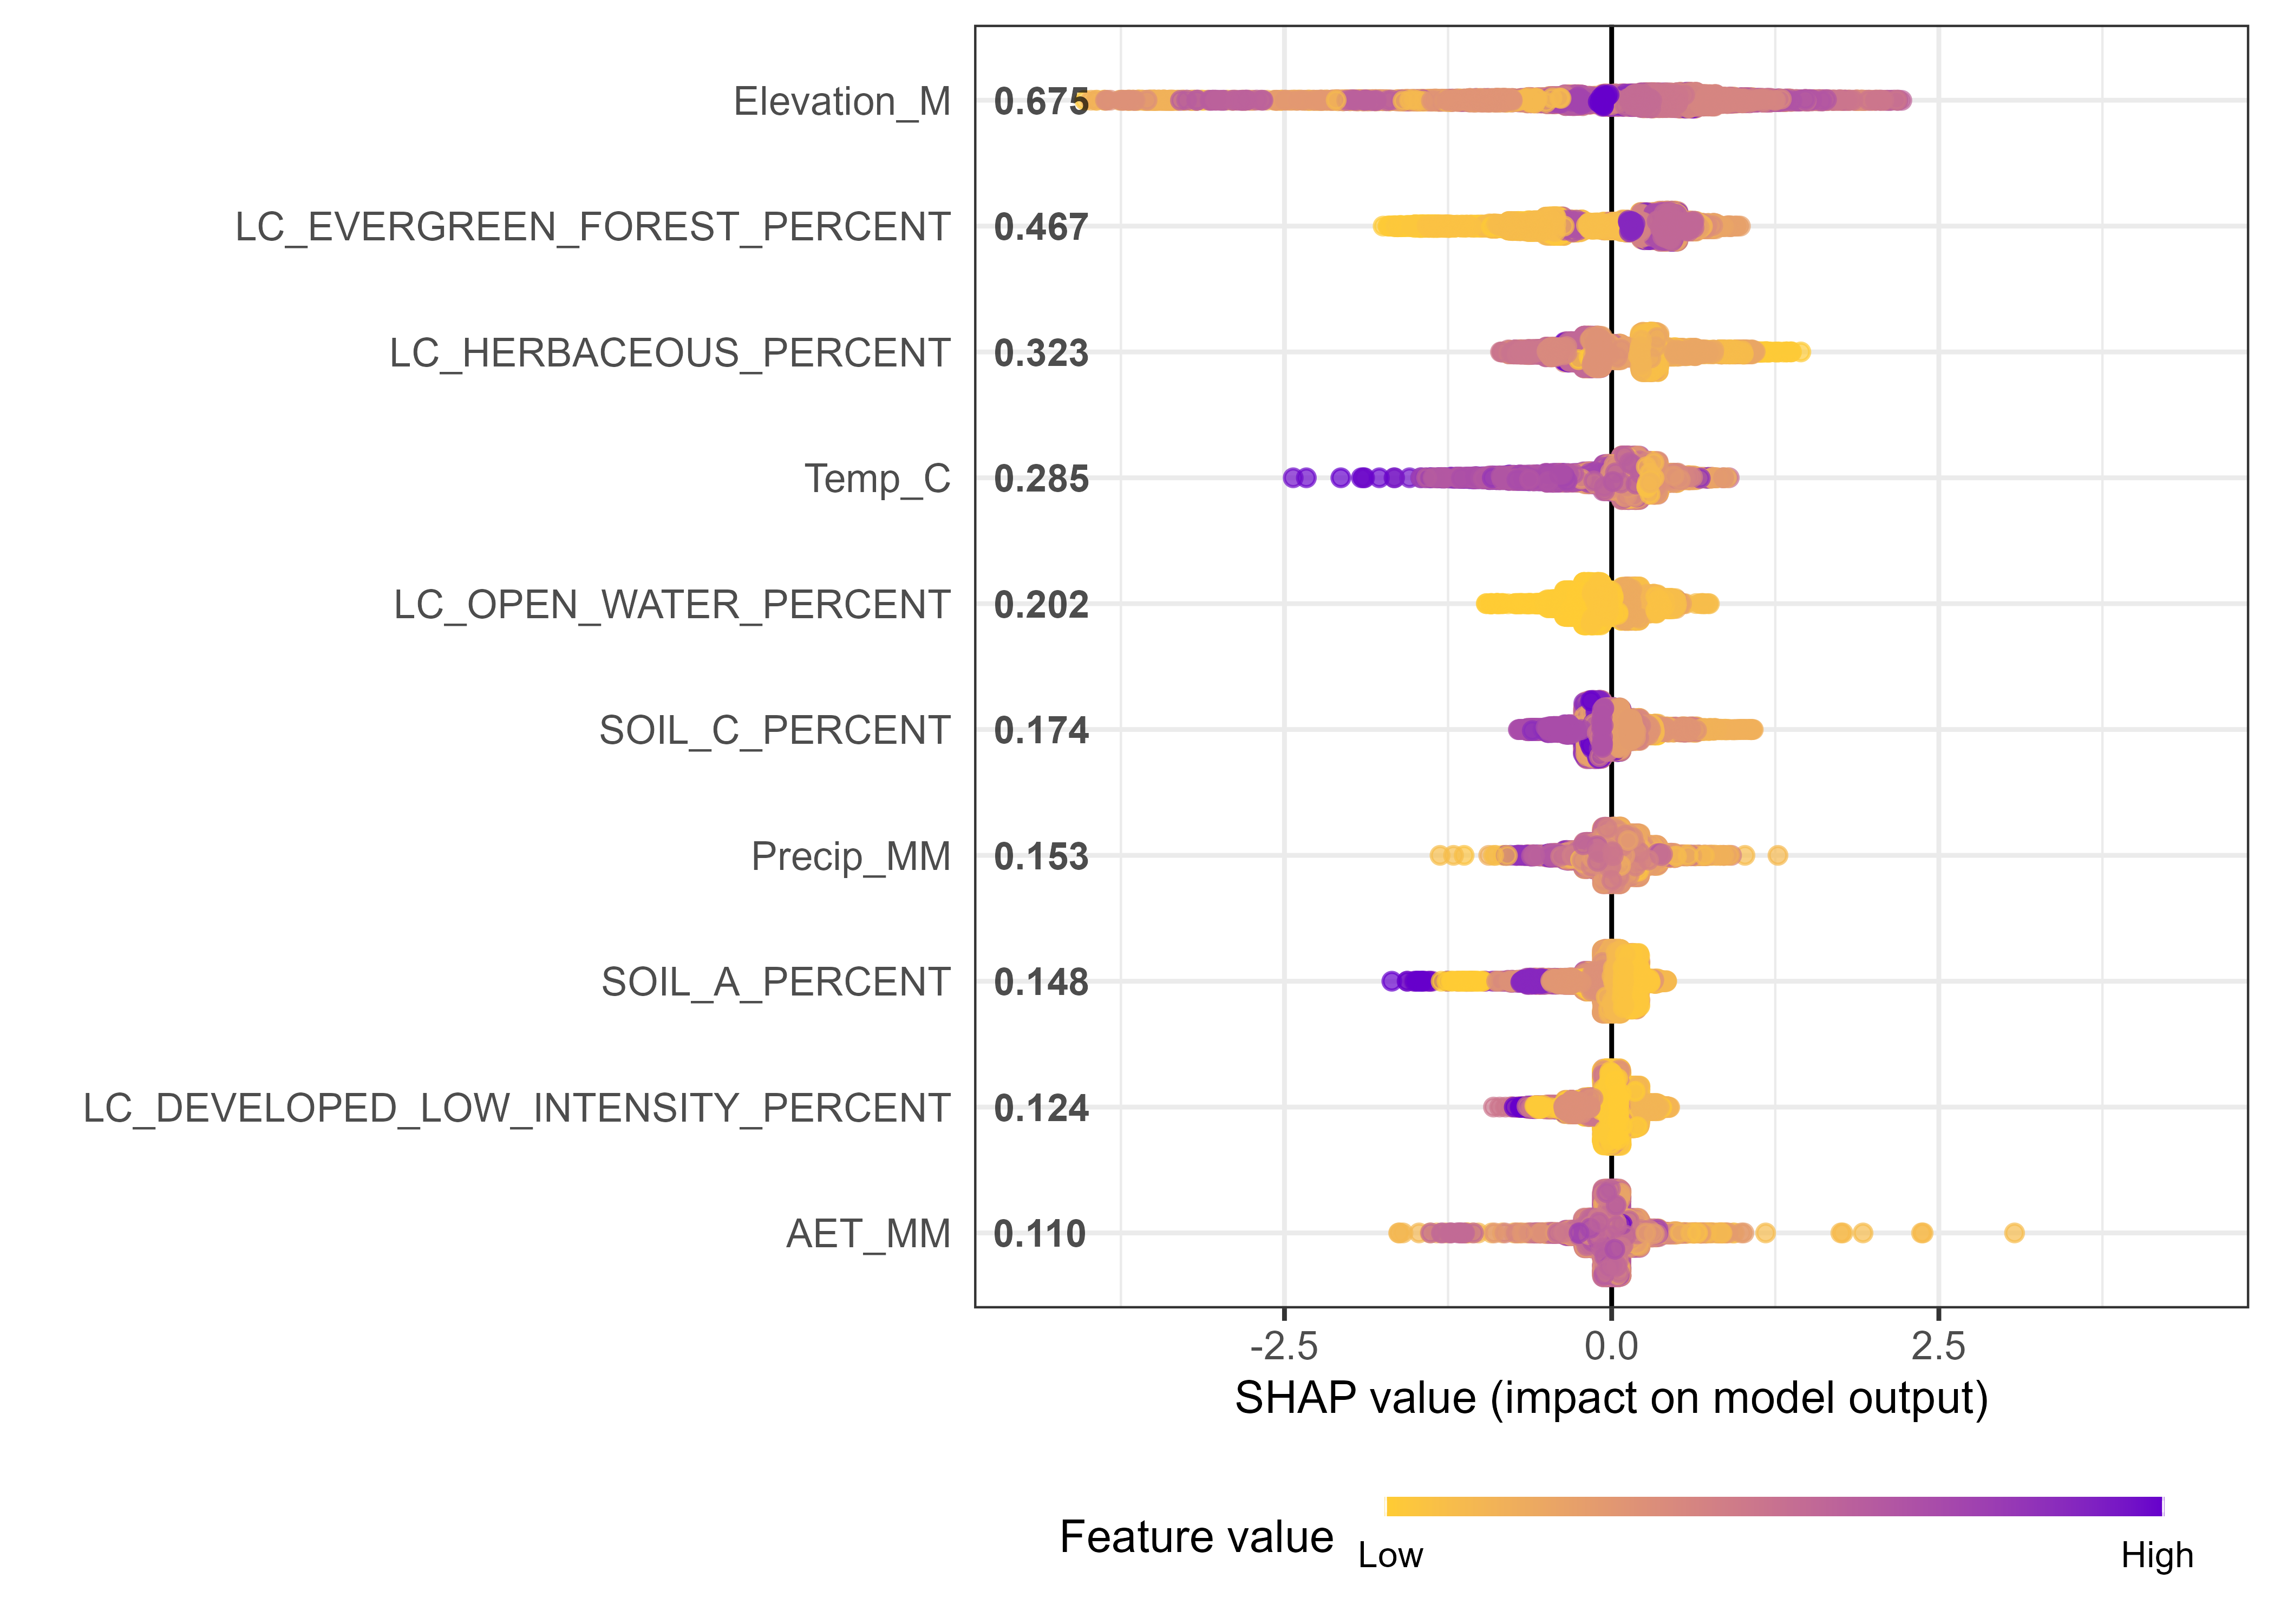
\includegraphics{images/shap_summary.png}

}

\caption{\label{fig-shap_values}SHAP value plot of features used in
final model. The number to the right of the feature name is the mean
absolute SHAP value. Land cover features are indicated by the percentage
of cover by each land cover type and soil types are defined by
hydrologic soil group.}

\end{figure}%

The ten most important features Figure~\ref{fig-shap_values} were
selected based on their SHAP values and used to train a subsequent model
Table~\ref{tbl-predictors}. This refined model demonstrated improved
performance and reduced computational time compared to the initial
model. The final model, trained on this optimized feature subset, was
ultimately used for the analysis presented here.

\subsection{Statistical Analyses}\label{statistical-analyses}

Statistical analyses were conducted on annual BFI values from
instrumented streamgages to identify site-specific temporal trends using
the Mann--Kendall nonparametric trend test
\citep{kendall1970, mann1945nonparametric}. This test detects monotonic
trends in non-normally distributed data and assumes the absence of
autocorrelation. This test is widely used in hydrologic trend studies
\citep{ficklin2016, ayers2019, woodhouse_udall22}.

To account for potential autocorrelation in annual BFI time series at
each instrumented site, we applied the Durbin--Watson test
\citep{durbin1950testing}. Four streamgages exhibited significant
autocorrelation; these sites were excluded from the trend analysis to
avoid inflated variance in the Mann--Kendall statistic and potential
bias in trend detection \citep{MK_Hamed1998}. As all autocorrelated
series were removed, pre-whitening using the Hamed--Rao method was
unnecessary \citep{MK_Hamed1998}. Trends with a \(\alpha \le 0.05\) are
considered significant.

\section{Results}\label{results}

\subsection{Observed BFI in Gauged
Catchments}\label{observed-bfi-in-gauged-catchments}

The long-term BFI for the 205 gauged reaches across Arizona is
illustrated in Figure~\ref{fig-instrumented-bfi} . The long-term mean
BFI is 0.32, indicating that \textasciitilde32\% of long-term streamflow
in Arizona likely originates from groundwater discharge and other
delayed sources. The highest long-term BFI values (\textgreater0.9) are
found along the Grand Canyon in northwestern Arizona, where highly
karstic geology facilitates rapid subsurface flow to surface water and
spring outlets \citep{chambless_deep-karst_2023}. High long-term BFI
values (\textgreater0.8) are also found at the spring-fed headwaters of
the Verde River and Fossil Creek, which have similar highly-karstic,
snowmelt-driven recharge areas.

The stream reaches of the Little Colorado River Basin (northeastern
Arizona) indicate low long-term BFI values (\textless{} 0.2). This is
likely due to low-yielding perched aquifers underlying the Defiance
Plateau in northeastern Arizona, which are hydrologically connected to
surface streams, while the high-yield, confined regional aquifer is much
deeper \citep{blanchard02}.

\begin{figure}

\centering{

\includegraphics{images/updated/BFI_Instrumented_20240404.png}

}

\caption{\label{fig-instrumented-bfi}Long-term BFI for the period of
record from instrumented stream flow data.}

\end{figure}%

\subsubsection{Trends in BFI}\label{sec-bfi-trends}

Trends in long-term BFI over the period of record for each streamgage
are illustrated in Figure~\ref{fig-instrumented-trend} and summarized in
Table~\ref{tbl-trends}. Long-term BFI trends were assessed at all
instrumented sites using the Mann--Kendall test. As BFI quantifies the
proportion of streamflow attributed to base flow, its long-term trends
inherently reflect changes in subsurface contributions relative to total
flow. A 72.2\% coincidence rate between significant base flow and BFI
trends supports the interpretation that changes in BFI are largely
driven by underlying base-flow dynamics. Statistically significant
long-term BFI trends were observed across numerous sites, with spatial
variation highlighting regional differences in hydrologic response.

Figure~\ref{fig-instrumented-trend} illustrates the spatial variation in
long-term BFI trends across the study area. Statistically significant
decreasing trends are observed at 16.1\% of sites, while increasing
trends are found at 8.8\% of sites. No consistent regional patterns are
evident.

\begin{figure}

\centering{

\includegraphics{images/updated/BFITrends_20250404.png}

}

\caption{\label{fig-instrumented-trend}Trends in BFI over full period of
record for instrumented sites used in this study. Red downward (blue
upward) arrows indicate a decreasing (increasing) trend at a
significance level of 5\%. White circles represent sites with no
statistically significant trends.}

\end{figure}%

\subsubsection{Classification Trends}\label{classification-trends}

Classifications presented in Table~\ref{tbl-trends} were determined
based on precipitation regime, physiographic region, climate, and slope.
The dominant precipitation regime (monsoon vs.~snowmelt) was identified
by analyzing streamflow hydrographs for each station, focusing on peak
flow periods during the monsoon season (July--September) and the
snowmelt season (March--June). Physiographic region was assigned based
on which region the streamgage is located. Climate classifications were
defined as warm (above the long-term median temperature of Arizona),
cool (below the long-term median temperature), wet (above the long-term
median precipitation), and dry (below the long-term median
precipitation). Slope was categorized as high (above the median slope)
and low (below the median slope).

Statistically significant decreasing trends in long-term BFI were more
common than increasing trends across all site classifications
(Table~\ref{tbl-trends}). While decreasing trends dominate, both
increasing and decreasing trends are observed within each
classification. Monsoon-dominated regions exhibit a higher proportion of
significant negative trends (24.1\%) compared to snowmelt-dominated
regions (10.2\%), suggesting that monsoon-dominated systems are more
consistently correlated with declining long-term BFI. Among climate
classifications, warm-dry climates have the highest proportion of
negative trends (20.0\%), followed by warm-wet climates (19.4\%),
indicating that regions with higher temperatures are more prone to BFI
declines. Low-slope regions show a greater prevalence of negative trends
(20.4\%) compared to high-slope regions (11.8\%). This suggests that
flatter areas may be more susceptible to base-flow reductions,
potentially due to differences in hydrologic connectivity and recharge
dynamics.

\begin{longtable}[]{@{}
  >{\raggedright\arraybackslash}p{(\columnwidth - 10\tabcolsep) * \real{0.1667}}
  >{\raggedright\arraybackslash}p{(\columnwidth - 10\tabcolsep) * \real{0.1667}}
  >{\raggedright\arraybackslash}p{(\columnwidth - 10\tabcolsep) * \real{0.1667}}
  >{\raggedright\arraybackslash}p{(\columnwidth - 10\tabcolsep) * \real{0.1667}}
  >{\raggedright\arraybackslash}p{(\columnwidth - 10\tabcolsep) * \real{0.1667}}
  >{\raggedright\arraybackslash}p{(\columnwidth - 10\tabcolsep) * \real{0.1667}}@{}}
\caption{Comparison of trends for BFI for all sites split by various
classifications. Only sites with a significant (\(\alpha \le 0.05\))
trend are included here as established by a Mann-Kendall test for
monotonic trends across the full period of record. n is the number of
sites, n\_pos (n\_neg) is the number of sites with positive (negative)
trends, perc\_pos (perc\_neg) is the percentage of n with a positive
(negative) trend.}\label{tbl-trends}\tabularnewline
\toprule\noalign{}
\begin{minipage}[b]{\linewidth}\raggedright
\textbf{Classification Group}
\end{minipage} & \begin{minipage}[b]{\linewidth}\raggedright
\textbf{n}
\end{minipage} & \begin{minipage}[b]{\linewidth}\raggedright
\textbf{n\_pos}
\end{minipage} & \begin{minipage}[b]{\linewidth}\raggedright
\textbf{n\_neg}
\end{minipage} & \begin{minipage}[b]{\linewidth}\raggedright
\textbf{perc\_pos}
\end{minipage} & \begin{minipage}[b]{\linewidth}\raggedright
\textbf{perc\_neg}
\end{minipage} \\
\midrule\noalign{}
\endfirsthead
\toprule\noalign{}
\begin{minipage}[b]{\linewidth}\raggedright
\textbf{Classification Group}
\end{minipage} & \begin{minipage}[b]{\linewidth}\raggedright
\textbf{n}
\end{minipage} & \begin{minipage}[b]{\linewidth}\raggedright
\textbf{n\_pos}
\end{minipage} & \begin{minipage}[b]{\linewidth}\raggedright
\textbf{n\_neg}
\end{minipage} & \begin{minipage}[b]{\linewidth}\raggedright
\textbf{perc\_pos}
\end{minipage} & \begin{minipage}[b]{\linewidth}\raggedright
\textbf{perc\_neg}
\end{minipage} \\
\midrule\noalign{}
\endhead
\bottomrule\noalign{}
\endlastfoot
Precipitation - Monsoon Dominated & 87 & 8 & 21 & 0.092 & 0.241 \\
Precipitation - Snowmelt Dominated & 118 & 9 & 12 & 0.076 & 0.102 \\
Physiographic Region - Basin and Range & 156 & 14 & 26 & 0.090 &
0.167 \\
Physiographic Region - Colorado Plateau & 49 & 3 & 7 & 0.061 & 0.143 \\
Climate - Warm-Wet & 31 & 2 & 6 & 0.065 & 0.194 \\
Climate - Warm-Dry & 55 & 6 & 11 & 0.109 & 0.200 \\
Climate - Cool-Wet & 74 & 4 & 9 & 0.054 & 0.122 \\
Climate - Cool-Dry & 45 & 5 & 7 & 0.111 & 0.156 \\
Slope - High & 102 & 10 & 12 & 0.098 & 0.118 \\
Slope - Low & 103 & 7 & 21 & 0.068 & 0.204 \\
\end{longtable}

\subsubsection{Coincident Climate
Trends}\label{coincident-climate-trends}

Coincident trends are defined as those in which long-term BFI trends
match in direction with climate variable trends over the same period.
Results are summarized in Table~\ref{tbl-coincident-trends}. This
analysis includes both significant and non-significant trends, which is
appropriate where the influence of complex, interconnected processes may
not always manifest as statistically significant patterns over limited
observational periods \citep{ficklin2016}. Coincidence was highest with
precipitation (64.88\% for base flow; 53.17\% for BFI), followed by ETO
and then temperature. Temperature trends most often show an inverse
relationship---i.e., warming associated with declining BFI and base
flow.

Given the variations in the period of record across the instrumented
network (see Figure S2), we analyzed trends of long-term BFI in relation
to coincident trends in climate variables. Trends are classified as
coincident when the direction of the climate variable trend (positive or
negative) aligns with the trend observed in BFI
(Table~\ref{tbl-coincident-trends}).

\begin{longtable}[]{@{}lcc@{}}
\caption{Coincident trends of climate variables (ET\textsubscript{O},
precipitation, temperature) with BFI
trends.}\label{tbl-coincident-trends}\tabularnewline
\toprule\noalign{}
& \textbf{Climate Variable} & \textbf{Coincidence Percentage (\%)} \\
\midrule\noalign{}
\endfirsthead
\toprule\noalign{}
& \textbf{Climate Variable} & \textbf{Coincidence Percentage (\%)} \\
\midrule\noalign{}
\endhead
\bottomrule\noalign{}
\endlastfoot
BFI & ET\textsubscript{O} & 44.88 \\
& Precipitation & 53.17 \\
& Temperature & 47.32 \\
\end{longtable}

\subsection{BFI of Ungauged
Catchments}\label{bfi-of-ungauged-catchments}

\subsubsection{Model Validation}\label{model-validation}

Predicted values of annual BFI are plotted against observed values for
the entire period of record of the instrumented dataset in
Figure~\ref{fig-actual_predicted} . The agreement between ``out-of-bag''
predictions (blind cross-validation, treating each site as ungauged) and
observed values indicate strong model performance across the full
dataset (R\textsuperscript{2} = 0.764). The overall RMSE is 0.129 and
the overall percent bias (pbias) is -5.6\%.

Model performance metrics across various classifications are summarized
in Table~\ref{tbl-performance}. These metrics show consistent model
performance across spatial and climatic classifications. However, the
negative pbias values across all classifications indicate a systematic
underprediction of annual BFI. Categories with relatively lower
R\textsuperscript{2} and Nash-Sutcliffe Efficiency (NSE) values also
exhibit higher biases, reflecting weaker model performance in those
contexts.

\begin{figure}

\centering{

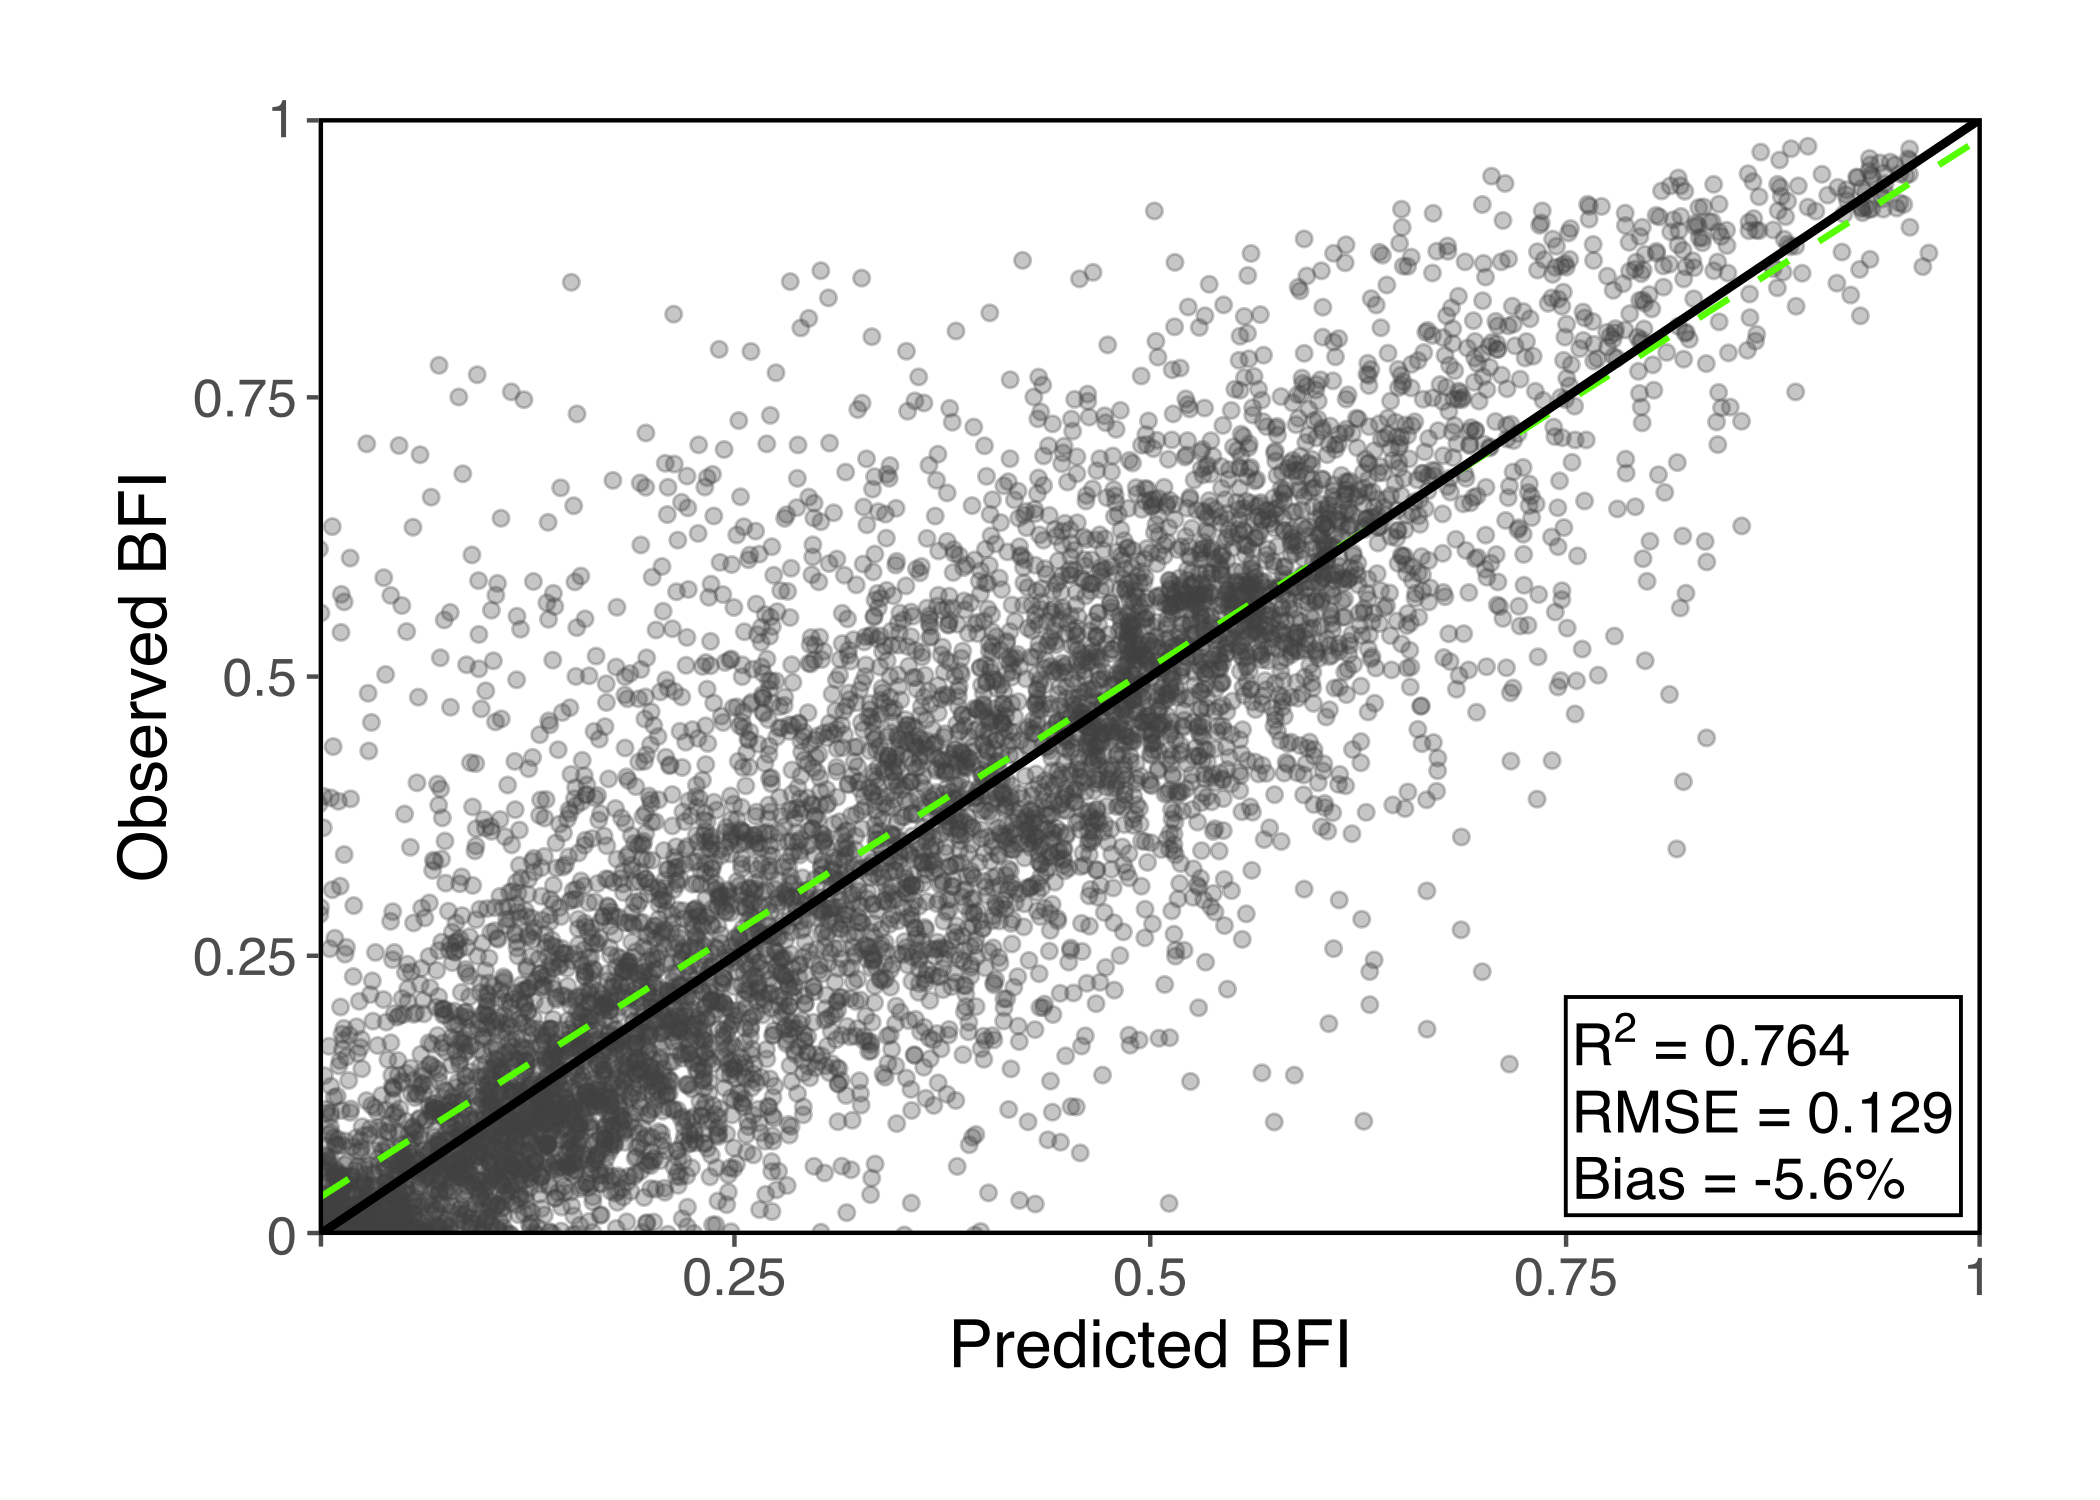
\includegraphics{images/actual-predicted.png}

}

\caption{\label{fig-actual_predicted}Linear relationship between
observed BFI and predicted BFI. The solid line is the 1:1 line, the
dashed, green line is regressed to the data.}

\end{figure}%

\begin{longtable}[]{@{}
  >{\raggedright\arraybackslash}p{(\columnwidth - 14\tabcolsep) * \real{0.1250}}
  >{\raggedright\arraybackslash}p{(\columnwidth - 14\tabcolsep) * \real{0.1250}}
  >{\raggedright\arraybackslash}p{(\columnwidth - 14\tabcolsep) * \real{0.1250}}
  >{\raggedright\arraybackslash}p{(\columnwidth - 14\tabcolsep) * \real{0.1250}}
  >{\raggedright\arraybackslash}p{(\columnwidth - 14\tabcolsep) * \real{0.1250}}
  >{\raggedright\arraybackslash}p{(\columnwidth - 14\tabcolsep) * \real{0.1250}}
  >{\raggedright\arraybackslash}p{(\columnwidth - 14\tabcolsep) * \real{0.1250}}
  >{\raggedright\arraybackslash}p{(\columnwidth - 14\tabcolsep) * \real{0.1250}}@{}}
\caption{Performance of model predictions for annual BFI for all sites
split by various classifications. n is number of observations,
R\textsuperscript{2} is the coefficient of determination of a linear
regression, MSE is mean-squared-error, RMSE is root-mean-squared-error,
MAE is mean-absolute-error, NSE is Nash-Sutcliffe efficiency, and pbias
is percent bias.}\label{tbl-performance}\tabularnewline
\toprule\noalign{}
\begin{minipage}[b]{\linewidth}\raggedright
\textbf{Classification Group}
\end{minipage} & \begin{minipage}[b]{\linewidth}\raggedright
\textbf{n}
\end{minipage} & \begin{minipage}[b]{\linewidth}\raggedright
\textbf{R2}
\end{minipage} & \begin{minipage}[b]{\linewidth}\raggedright
\textbf{MSE}
\end{minipage} & \begin{minipage}[b]{\linewidth}\raggedright
\textbf{RMSE}
\end{minipage} & \begin{minipage}[b]{\linewidth}\raggedright
\textbf{MAE}
\end{minipage} & \begin{minipage}[b]{\linewidth}\raggedright
\textbf{NSE}
\end{minipage} & \begin{minipage}[b]{\linewidth}\raggedright
\textbf{pbias}
\end{minipage} \\
\midrule\noalign{}
\endfirsthead
\toprule\noalign{}
\begin{minipage}[b]{\linewidth}\raggedright
\textbf{Classification Group}
\end{minipage} & \begin{minipage}[b]{\linewidth}\raggedright
\textbf{n}
\end{minipage} & \begin{minipage}[b]{\linewidth}\raggedright
\textbf{R2}
\end{minipage} & \begin{minipage}[b]{\linewidth}\raggedright
\textbf{MSE}
\end{minipage} & \begin{minipage}[b]{\linewidth}\raggedright
\textbf{RMSE}
\end{minipage} & \begin{minipage}[b]{\linewidth}\raggedright
\textbf{MAE}
\end{minipage} & \begin{minipage}[b]{\linewidth}\raggedright
\textbf{NSE}
\end{minipage} & \begin{minipage}[b]{\linewidth}\raggedright
\textbf{pbias}
\end{minipage} \\
\midrule\noalign{}
\endhead
\bottomrule\noalign{}
\endlastfoot
Climate - Monsoon Dominated & 3039 & 0.633 & 0.016 & 0.126 & 0.074 &
0.619 & -13.7 \\
Climate - Snowmelt Dominated & 4685 & 0.733 & 0.015 & 0.121 & 0.087 &
0.725 & -3.5 \\
PhysRegion - Basin\&Range & 6147 & 0.733 & 0.016 & 0.127 & 0.084 & 0.724
& -6.3 \\
PhysRegion - CO Plateau & 1577 & 0.846 & 0.011 & 0.104 & 0.073 & 0.843 &
-3.8 \\
Climate - Warm-Wet & 1506 & 0.693 & 0.014 & 0.117 & 0.077 & 0.685 &
-8.2 \\
Climate - Warm-Dry & 2351 & 0.693 & 0.022 & 0.147 & 0.092 & 0.675 &
-11.9 \\
Climate - Cool-Wet & 2350 & 0.738 & 0.011 & 0.106 & 0.078 & 0.736 &
-1.7 \\
Climate - Cool-Dry & 1517 & 0.831 & 0.012 & 0.111 & 0.078 & 0.827 &
-4.3 \\
Slope - High & 3795 & 0.776 & 0.012 & 0.111 & 0.079 & 0.771 & -3.3 \\
Slope - Low & 3929 & 0.724 & 0.018 & 0.133 & 0.085 & 0.713 & -9.1 \\
\end{longtable}

\subsubsection{Predictor Importance}\label{sec-predictor-importance}

The predictors used to estimate annual BFI at ungauged sites were
evaluated for their importance in the final XGBoost model, as
illustrated in Figure~\ref{fig-shap_values}. The most influential
feature for predicting annual BFI is basin elevation. While elevation
itself does not directly affect base-flow characteristics, it has
consistently been identified as a key predictor in previous BFI studies
\citep{singh2018, beck2013}. The importance of elevation aligns with
findings from \citet{beck2013}, highlighting its role as a proxy for
climate variables such as temperature, precipitation, and snowpack
duration. Seasonal snowpack duration, in particular, has been shown to
strongly correlate with springflow and groundwater recharge in this
region \citep{donovan_karst_2022}.

Land cover and land use predictors also play a significant role in
annual BFI estimation. Analysis of SHAP values indicates that a higher
percentage of evergreen forest positively influences BFI predictions,
while higher proportions of shrubland and developed land exert a
negative influence. Similarly, hydrologic soil types show distinct
trends in their impact on BFI. Soil Type C, characterized by moderately
high runoff potential (20-40\% clay), tends to negatively influence BFI.
In contrast, Soil Type A, which has low runoff potential and facilitates
rapid water infiltration, exhibits a mixed influence \citep{nrcs2009}.

\subsubsection{Predicted BFI in Ungauged
Basins}\label{predicted-bfi-in-ungauged-basins}

The regionalized (HUC-8) long-term BFI (1991--2020) is shown in
Figure~\ref{fig-bfi-huc}. Basins with high long-term BFIs, such as those
along the Grand Canyon in the northwestern part of the study area,
indicate greater surface water and groundwater interaction. Elevated BFI
values are also observed along portions of the Mogollon Rim, a heavily
forested region with high precipitation that marks the transition
between physiographic regions. Additionally, headwater regions of
perennial rivers tend to exhibit higher long-term BFI values. In
contrast, low long-term BFI values are found in areas like the Defiance
Plateau in northeastern Arizona and the arid southern regions of the
state.

\begin{figure}

\centering{

\includegraphics{images/BFI_HUC8_20250525.png}

}

\caption{\label{fig-bfi-huc}Predicted long-term BFI values for 8-digit
HUC (1991-2020). Bolded HUCs indicate those without a streamgage.}

\end{figure}%

\section{Discussion}\label{discussion}

Several previous studies have examined regional and continental patterns
of BFI, offering useful context for our findings despite limited
geographic overlap. \citet{beck2013} developed a global map of BFI using
an artificial neural network trained on 1,862 U.S. streamgages from the
MOPEX dataset \citep{mopex_2006}. Only ten of these gauges overlap with
our Arizona study area, limiting direct comparison. Nonetheless, the
spatial distribution of BFI in Arizona from \citet{beck2013} shows
general agreement with our regional patterns. The higher BFI values
reported by \citet{beck2013} may reflect the influence of their
global-scale ANN model and associated generalizations. Similarly,
\citet{ayers2022} examined base-flow dynamics using GAGES-II sites
across CONUS, but their study included few gauges within Arizona. While
exact locations are not specified, their published figures suggests
regional agreement with our estimated BFI distributions.
\citet{santhi2008} employed interpolation methods for regional base-flow
estimation across CONUS, but specific gauge locations or data are not
available limiting comparison.````

In terms of long-term trends, our results align directionally with
\citet{ayers2022} , who found consistent monthly declines in base flow
from 1989--2019 across the U.S. Southwest. Although our analysis focused
on long-term trends in annual BFI, we observed a similar imbalance: 16\%
of sites showed significant decreasing trends compared to 8\% with
increasing trends. While we do not directly replicate their monthly
analysis, the directional agreement supports the broader conclusion that
groundwater contributions to streamflow are declining in many parts of
the region.

The existing streamgage networks in Arizona are limited for base-flow
analyses by their design and monitoring objectives. While the number of
streamgages has increased to meet regulatory imperatives, such as those
driven by the Clean Water Act, many gauges prioritize peak flow
monitoring rather than low-flow conditions critical for base-flow
studies \citep{flood-control2020}. Newer non-USGS gauges, such as those
installed by flood control districts (e.g., the ALERT system), are
generally tailored for flood detection rather than monitoring sustained
base flow. Recent USGS installations focus on addressing in-stream flow
rights and future monitoring improvements, though low-flow capabilities
remain limited.

This study addresses these monitoring gaps through an analysis of
observed BFI at instrumented streamgages, highlighting
groundwater-surface water interactions within Arizona's arid and
semi-arid landscapes. Observed spatial patterns in BFI clearly align
with known hydrogeological and climatic variations. High long-term BFI
values coincide with areas characterized by spring-fed streams and
pronounced physiographic transitions, such as the Grand Canyon and
Mogollon Rim. Conversely, lower observed BFI values correspond to
regions with limited groundwater contributions, notably the Defiance
Plateau and southern Arizona, emphasizing vulnerability in these arid
environments. A trend of high BFI in upstream reaches to lower BFI in
downstream reaches Figure~\ref{fig-instrumented-bfi} likely indicates a
transition from zones of groundwater discharge to zones of groundwater
recharge and may indicate a transition from gaining stream reaches to
losing stream reaches \citep{winter2007}.

Analysis of trends at instrumented sites revealed a predominance of
declining long-term BFI values, particularly within monsoon-dominated
precipitation regimes, warm-dry climates, and low-slope basins. These
negative trends likely reflect intensified climate stress, highlighting
areas most vulnerable to groundwater depletion and surface-water
scarcity. Precipitation was identified as the primary driver influencing
base-flow variability, with temperature and evapotranspiration trends
adding complexity. The weaker correlation between temperature and BFI
trends suggests that temperature impacts are moderated by other
environmental factors, underscoring the need for integrated climate and
land-management strategies to protect groundwater-dependent ecosystems.

Given the limited coverage provided by existing gauges, a common issue
in arid and semi-arid regions globally \citep{krabbenhoft-2022}, we
utilized a machine learning approach to estimate annual BFI in ungauged
catchments. The regional model exhibited strong predictive capability
(overall R²=0.764), though systematic underprediction (negative pbias)
was noted, particularly in monsoon-dominated and warm-dry climates.
These biases suggest areas for improvement in model performance,
potentially through the incorporation of additional predictors or more
refined regional hydrologic representations. Although creating separate
regional models (by physiographic region) was explored to enhance
predictive accuracy, the state-wide model consistently outperformed
these regionalized approaches, emphasizing the advantage of a
comprehensive, state-wide dataset.

Elevation emerged as the most significant predictor, reinforcing its
established role as a proxy for climate conditions influencing
groundwater recharge. This aligns with findings from previous studies
conducted in diverse landscapes, including New Zealand
\citep{singh2018}, across CONUS \citep{santhi2008}, and globally
\citep{beck2013}. The mixed influence observed for Soil Type A indicates
complexity in infiltration dynamics, suggesting that future research
could benefit from explicitly incorporating temporal variables such as
snowpack duration, soil moisture, and detailed land-cover
characteristics.

\section{Conclusions}\label{conclusions}

The long-term average BFI across Arizona is approximately 0.32,
highlighting that groundwater discharge significantly contributes to
surface water flows but exhibits substantial spatial variability. Our
machine learning model (XGBoost) effectively predicts annual BFI in
ungauged catchments (R² = 0.764), primarily driven by basin elevation,
land cover, and hydrologic soil characteristics. Regions such as the
Grand Canyon and Mogollon Rim exhibit the highest long-term BFI values,
signifying robust groundwater-surface water interactions, whereas areas
such as the Defiance Plateau and southern Arizona show consistently
lower BFI values, reflecting limited groundwater contributions.

Analysis of temporal trends indicates a prevailing pattern of declining
long-term BFI across the region, particularly in monsoon-dominated,
warm-dry, and low-slope areas. Precipitation emerged as the strongest
driver of base-flow variability, while temperature and
evapotranspiration added additional layers of complexity. The observed
trends underscore the sensitivity of Arizona's hydrological systems to
climatic variability and suggest increasing vulnerability under
projected climate change scenarios and other stresses to aquifers, such
as increased groundwater pumping.

This research highlights critical limitations in Arizona's current
streamgage network for monitoring base-flow processes, suggesting a need
for targeted investments in instrumentation capable of capturing
low-flow dynamics. Additionally, the demonstrated success of our
modeling framework accentuates its broader applicability to similarly
data-scarce dryland regions globally, providing a valuable tool for
water resource management and climate adaptation strategies. By
improving our understanding of groundwater-surface water interactions
under changing climatic conditions, this study contributes substantially
to addressing hydrological uncertainties in arid and semi-arid
environments.


\renewcommand\refname{References}
  \bibliography{references.bib}



\end{document}
